\chapter{Hello PHP}

\section{PHP Standard Recommendation (PSR)}

PSR เป็นมาตรฐานการเขียนโค้ด PHP โดย PHP Framework Interop Group (PHP-FIG) 
เพื่อให้การเขียนโค้ดระหว่างโปรเจคทำงานร่วมกันได้

PSR-4 เป็นหัวข้อลำดับหมายเลข 4 ในมาตรฐาน PSR ซึ่งนำ Autoload 
มาช่วยในการเรียกใช้คลาสที่เป็น namespace จากเดิมที่ต้องเรียกใช้คลาสด้วยคำสั่ง 
\mintinline{php}{require "dir/YourClass.php"} 
เปลี่ยนเป็น \mintinline{php}{use <namespace>\<YourClass>} แทน 
(หัวข้อ PSR อื่น ศึกษาเพิ่มเติมได้ที่ https://www.php-fig.org/psr/) 
สิ่งที่ต้องใช้ในการเขียนโค้ดตามมาตรฐาน PSR-4 คือ PHP 5.3 ขึ้นไป 
(ปัจจุบัน กันยายน 2563 เป็นเวอร์ชัน PHP 7.4) และ 
Composer (https://getcomposer.org/)

\section{Composer}

Composer เป็นเครื่องมือช่วยจัดการแพคเกจหรือไลบรารีของภาษา PHP 
รวมถึงช่วยจัดการโปรเจคที่เขียนขึ้นเองได้ด้วย การติดตั้ง Composer 
ให้ดูที่ https://getcomposer.org/download/ 

\subsection{การติดตั้ง local development environment สำหรับระบบปฏิบัติการ Windows}
แนะนำให้ลงโปรแกรม Laragon 
(ดาวน์โหลดที่ https://laragon.org/download/ 
เลือก Edition Laragon Full)

Laragon เป็นโปรแกรมจำลองสภาพแวดล้อมการทำงานของเครื่องเป็น 
development environment ซึ่งรองรับการเขียน Web Application 
เพราะมี Web Server, Database Server และรองรับภาษาในการเขียน 
Web Application หลายภาษา รวมถึงมี Composer ติดตั้งมาด้วย

การใช้งาน command line interface tool ให้ใช้งานผ่าน terminal ใน Laragon

\subsection{การติดตั้ง local development environment สำหรับระบบปฏิบัติการ OSX}

1. ติดตั้ง Homebrew - The Missing Package Manager for MacOS (or Linux) (ดูวิธีการติดตั้งที่ https://brew.sh/)

2. ติดตั้ง Homebrew Services
\begin{cli}{cli:ch1:01}
    brew tap homebrew/services
\end{cli}

3. ติดตั้ง PHP, Composer, MySQL และ NodeJS
\begin{cli}{cli:ch1:02}
    brew install php
    brew install composer
    brew install mysql
    brew install node
\end{cli}

4. ตั้งค่า PATH ของ Composer

4.1 แก้ไขไฟล์ \mintinline{bash}{~/.bash_profile} โดยเพิ่มบรรทัดคำสั่ง \\
\mintinline{bash}{export PATH="~/.composer/vendor/bin:$PATH"}  

4.2 บันทึกไฟล์ แล้ว restart terminal

5. ติดตั้ง Valet (https://laravel.com/docs/8.x/valet)
\begin{cli}{cli:ch1:03}
composer global require laravel/valet
valet install
\end{cli}

6. กำหนด root document directory (https://laravel.com/docs/8.x/valet\#serving-sites)
\begin{cli}{cli:ch1:04}
    mkdir ~/sites
    cd ~/sites
    valet park
\end{cli}

7. คำสั่ง start MySQL
\begin{cli}{cli:ch1:05}
    brew services start mysql
\end{cli}

\section{การใช้งาน Composer เบื้องต้น}

1. สร้าง directory \mintinline{bash}{mypsr} ใน root document directory และสร้าง directory ย่อย \mintinline{bash}{src}

2. สร้างไฟล์ \mintinline{bash}{composer.json} ใน directory \mintinline{bash}{mypsr}
\begin{figure}[h!]
    \centering
    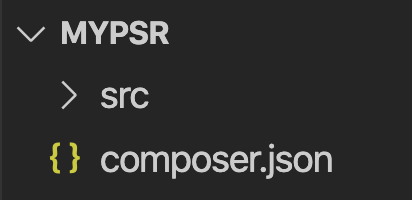
\includegraphics[width=0.3\textwidth]{images/ch1/01.png}
    \label{fig:ch1.1-mypsr-folder}
\end{figure}\\
โดยมีโค้ดดังนี้
\begin{code}{javascript}{/mypsr/composer.json}{code:ch1:composer}
    {
        "autoload": {
            "psr-4": {
                "App\\": "src/"
            }
        }
    }
\end{code}

3. ใช้ command line interface tool (terminal) เปลี่ยน current directory เป็น \mintinline{bash}{mypsr}
(เพื่อเข้าถึงไฟล์ \mintinline{bash}{composer.json}) จากนั้นใช้ composer สร้าง script สำหรับการใช้งาน autoload ด้วยคำสั่ง
\begin{cli}{cli:ch1:06}
    cd mypsr
    composer dump-autoload
\end{cli}

\newpage

4. สังเกตว่าจะมี directory \mintinline{bash}{vendor} ซึ่งในนั้นจะมีไฟล์ \mintinline{bash}{autoload.php}
และมี directory \mintinline{bash}{composer}
\begin{figure}[h!]
    \centering
    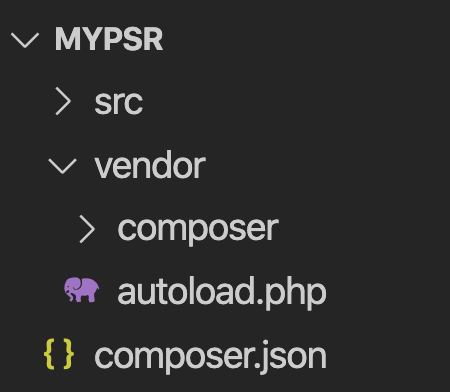
\includegraphics[width=0.3\textwidth]{images/ch1/02.png}
    \label{fig:ch1.2-mypsr-folder}
\end{figure}\\

5. สร้างตัวอย่างคลาส Foo ใน directory \mintinline{bash}{src}

\begin{code}{php}{/mypsr/src/Foo.php}{code:ch1:mypsr/src/Foo}
    <?php
    namespace App;
    
    class Foo {
        public function bar($message) {
            return "Hello {$message}";
        }
    }
\end{code}

6. สร้างไฟล์ index.php ใน directory \mintinline{bash}{mypsr}
\begin{code}{php}{/mypsr/index.php}{code:ch1:mypsr/src/Foo}
    <?php
    require 'vendor/autoload.php';

    use App\Foo;

    $foo = new Foo();
    echo $foo->bar('PSR-4');

\end{code}

\newpage

7. ทดสอบรันไฟล์ index.php ผ่าน terminal

\begin{cli}{cli:01}
    php index.php
\end{cli}

\begin{out}{out:01}
    Hello PSR-4
\end{out}

\subsection{ข้อควรจำ}
1. ทุกครั้งที่มีการแก้ไขไฟล์ \mintinline{bash}{composer.json} (เช่น เพิ่ม namespace ให้ Directory ใหม่) 
จะต้องสั่ง \mintinline{bash}{composer dump-autoload} ใหม่

2. สามารถสร้าง Directory ย่อย ใน Directory ที่กำหนด namespace ไว้แล้ว 
โดยไม่ต้องสั่ง dump-autoload เช่น สร้างคลาส FooBar 
ในไฟล์ \mintinline{bash}{src/Utilities/Helper/FooBar.php} 
ต้องกำหนด namespace ของคลาส FooBar เป็น \mintinline{php}{App\Utilities\Helper}

3. สังเกตว่า namespace ใช้ Backslash (\mintinline{bash}{\}) เป็นตัวคั่น ไม่ใช่ Slash (/) และไม่มี .php ในตอนที่ use class